% Asset ID: FAS2ProductMomentCorrelationCoefficientTikZ-001
% Unit: FAS2
% Topic code: FAS2-BIV
% Topic ID: FAS2ProductMomentCorrelationCoefficient
% Related lesson file: FAS2_product_moment_correlation_coefficient_lesson.md
% Related lesson section: # 9. Visual Asset Integration
% Used placeholder:
% [VISUAL PLACEHOLDER: FAS2ProductMomentCorrelationCoefficientTikZ-001 | Source: Transcript warning that r does not measure steepness | Insert from tikz/FAS2ProductMomentCorrelationCoefficientTikZ-001.tex | Purpose: Show that r measures closeness to a straight line, not gradient. Description: Two exact straight-line data sets with different gradients but the same perfect positive correlation r = 1.]
% Source: Teacher transcript warning that r measures closeness to a straight line, not steepness.
% Purpose: Show that two data sets can both have r = 1 even when their gradients are different.

\documentclass[tikz,border=8pt]{standalone}
\usepackage{amsmath}
\usepackage{xcolor}
\definecolor{Canvas}{HTML}{FAF9F6}
\definecolor{Ink}{HTML}{2C2C2E}
\definecolor{LineSoft}{HTML}{E5E5EA}
\definecolor{Gold}{HTML}{C5A059}
\definecolor{Blush}{HTML}{FBEFEF}
\begin{document}
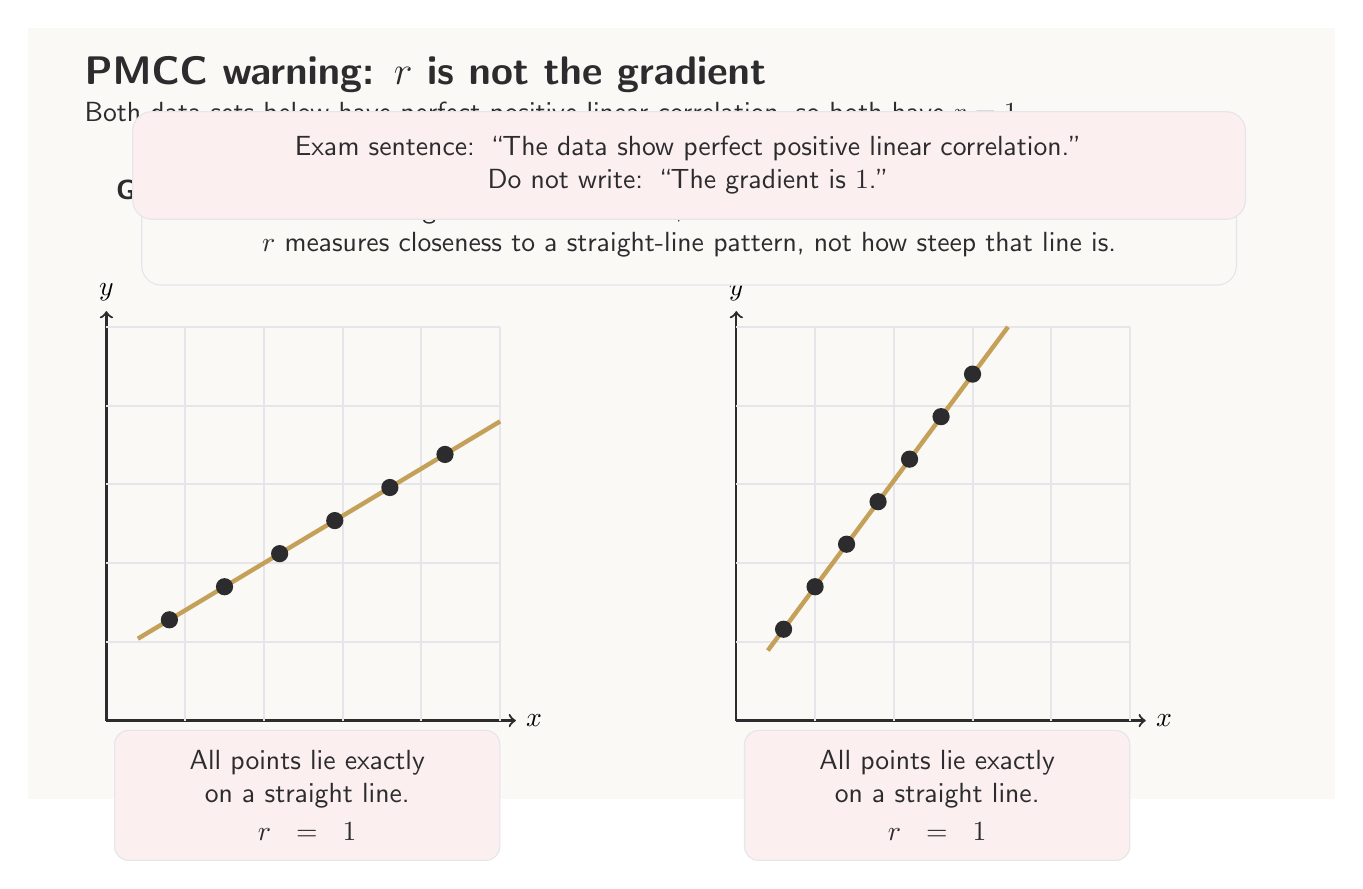
\begin{tikzpicture}[font=\sffamily,axis/.style={->, thick, draw=Ink},guide/.style={draw=LineSoft, line width=0.7pt},data/.style={circle, fill=Ink, inner sep=2.2pt},goldline/.style={draw=Gold, line width=1.6pt},note/.style={rounded corners=5pt,draw=LineSoft,fill=Blush,text=Ink,align=center,inner sep=7pt}]
\fill[Canvas] (-1.0,-1.0) rectangle (15.6,8.8);
\node[anchor=west, text=Ink, font=\sffamily\bfseries\Large] at (-0.4,8.2) {PMCC warning: \(r\) is not the gradient};
\node[anchor=west, text=Ink, font=\sffamily\normalsize] at (-0.4,7.7) {Both data sets below have perfect positive linear correlation, so both have \(r=1\).};
\begin{scope}[shift={(0,0)}]
\node[anchor=west, text=Ink, font=\sffamily\bfseries] at (0,6.7) {Gentle positive line};
\draw[axis] (0,0) -- (5.2,0) node[right] {\(x\)}; \draw[axis] (0,0) -- (0,5.2) node[above] {\(y\)};
\foreach \x in {1,2,3,4,5} {\draw[guide] (\x,0) -- (\x,5);} \foreach \y in {1,2,3,4,5} {\draw[guide] (0,\y) -- (5,\y);} 
\draw[goldline] (0.4,1.04) -- (5,3.8);
\foreach \x/\y in {0.8/1.28,1.5/1.70,2.2/2.12,2.9/2.54,3.6/2.96,4.3/3.38} {\node[data] at (\x,\y) {};}
\node[note, text width=4.4cm] at (2.55,-0.95) {All points lie exactly on a straight line.\\[2pt]\(\therefore r=1\)};
\end{scope}
\begin{scope}[shift={(8.0,0)}]
\node[anchor=west, text=Ink, font=\sffamily\bfseries] at (0,6.7) {Steep positive line};
\draw[axis] (0,0) -- (5.2,0) node[right] {\(x\)}; \draw[axis] (0,0) -- (0,5.2) node[above] {\(y\)};
\foreach \x in {1,2,3,4,5} {\draw[guide] (\x,0) -- (\x,5);} \foreach \y in {1,2,3,4,5} {\draw[guide] (0,\y) -- (5,\y);} 
\draw[goldline] (0.4,0.89) -- (3.45,5.0);
\foreach \x/\y in {0.6/1.16,1.0/1.70,1.4/2.24,1.8/2.78,2.2/3.32,2.6/3.86,3.0/4.40} {\node[data] at (\x,\y) {};}
\node[note, text width=4.4cm] at (2.55,-0.95) {All points lie exactly on a straight line.\\[2pt]\(\therefore r=1\)};
\end{scope}
\node[rounded corners=7pt,draw=LineSoft,fill=Canvas,text=Ink,align=center,inner sep=10pt,text width=13.2cm] at (7.4,6.25) {The gradients are different, but the PMCC is the same.\\ \(r\) measures closeness to a straight-line pattern, not how steep that line is.};
\node[rounded corners=7pt,draw=LineSoft,fill=Blush,text=Ink,align=center,inner sep=9pt,text width=13.5cm] at (7.4,7.05) {Exam sentence: ``The data show perfect positive linear correlation.''\\ Do not write: ``The gradient is \(1\).''};
\end{tikzpicture}
\end{document}
